%-----------------------------------------------------------------------------%
\chapter{METODE PENELITIAN}
%-----------------------------------------------------------------------------%

%
\vspace{4.5pt}

\begin{flushleft}
   \begin{justify}
      \section{Alur Penelitian}
      Langkah-langkah penelitian yang akan dilakukan sebagai bagian dari penelitian ini dapat dilihat pada Gambar 3.1
      \begin{figure}[ht]
         \centering
         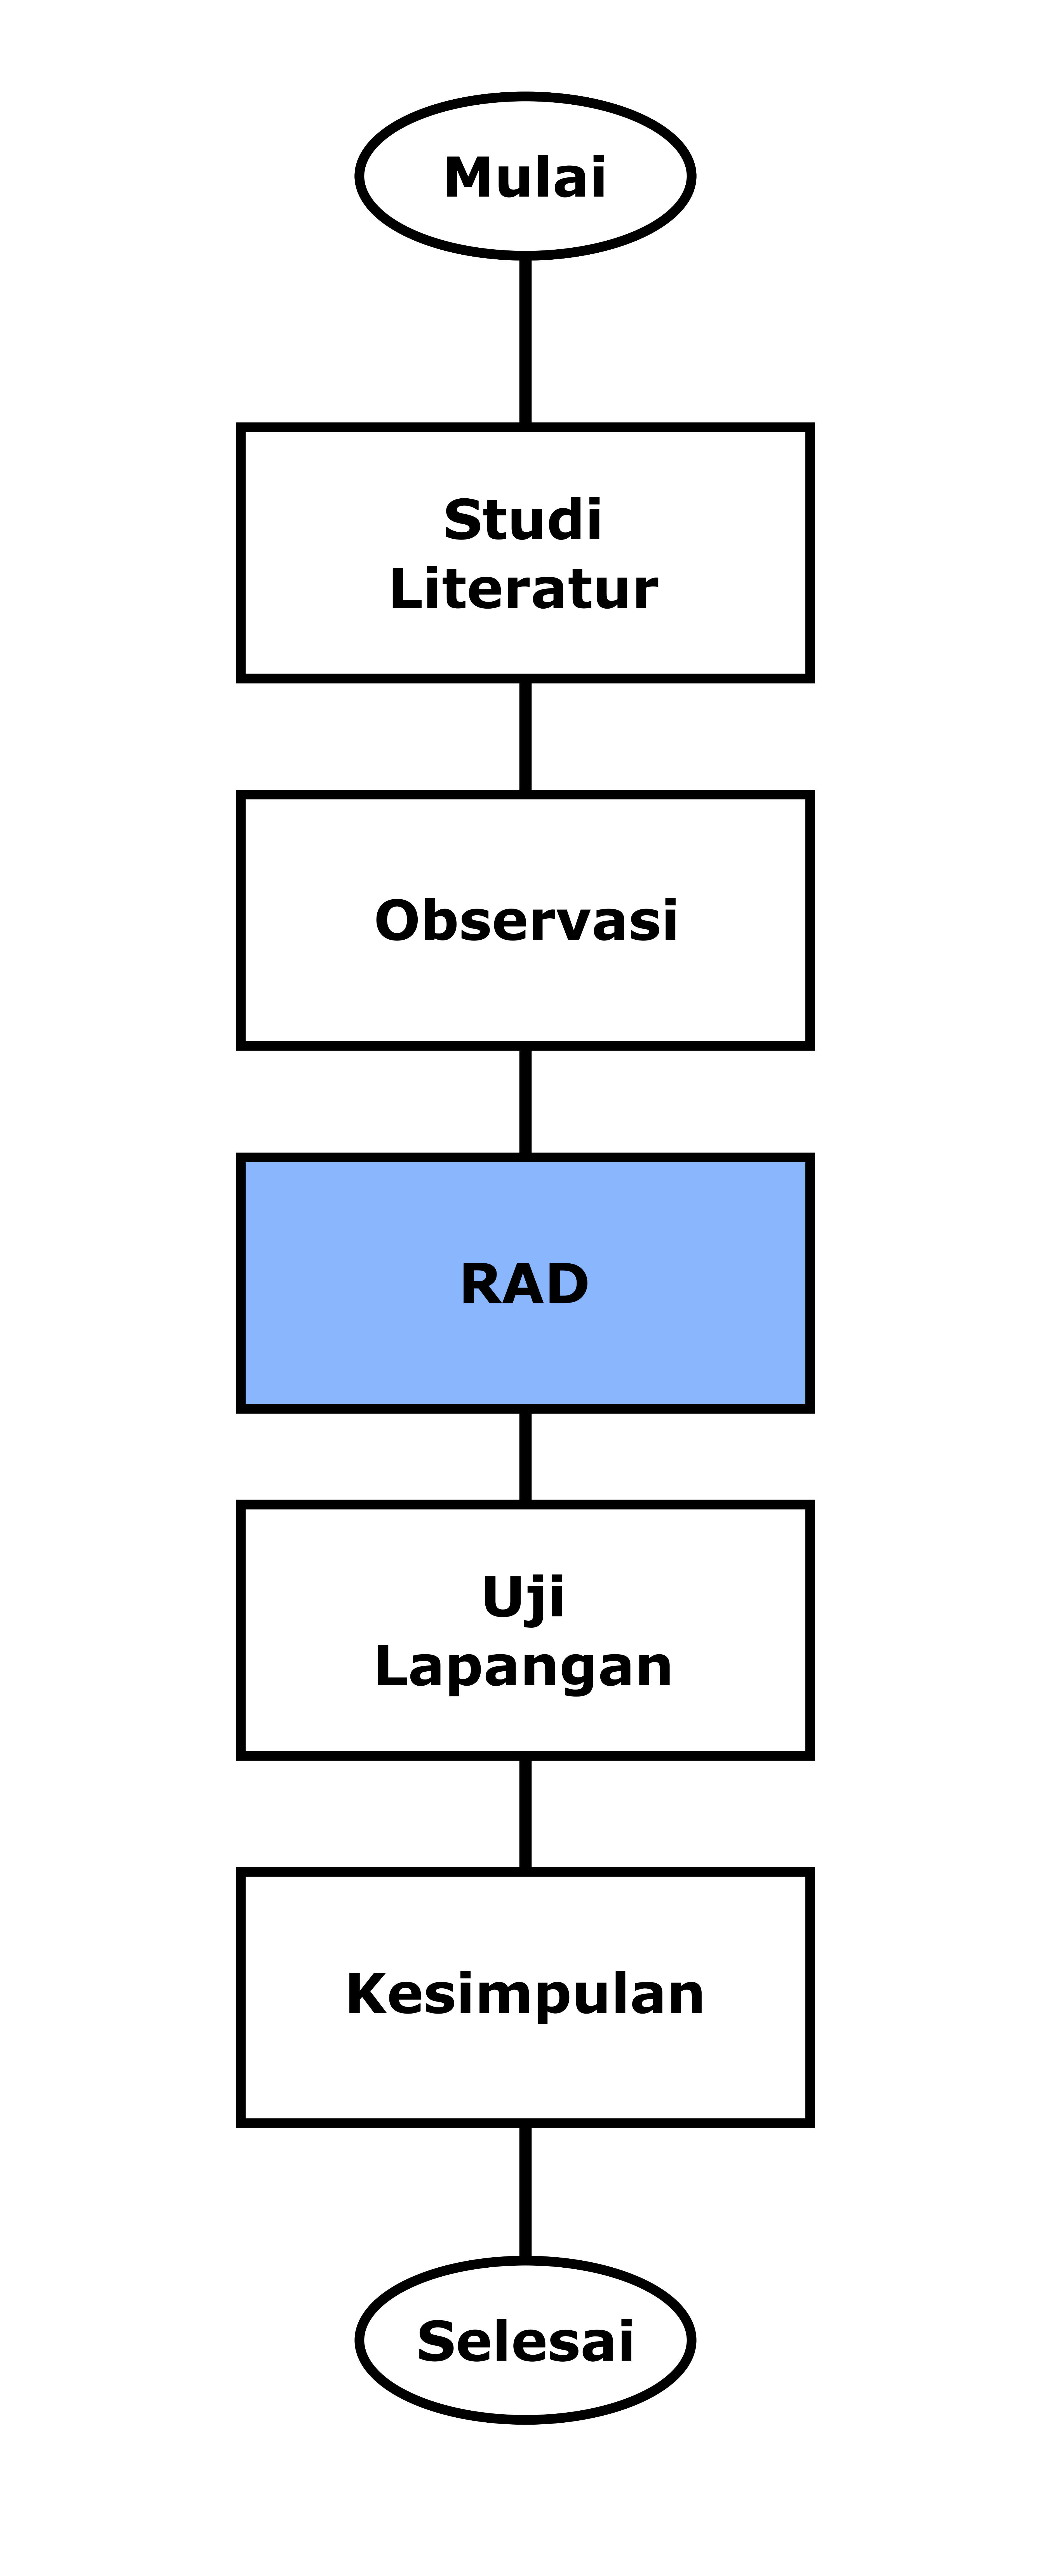
\includegraphics[width=6cm]{images/alur_penelitian.png}\\
         \caption{Alur Penelitian}
     \end{figure}

      \section{Penjabaran Langkah Penelitian}
       Berikut ini merupakan prosedur penelitian yang dilakukan.
         \subsection{Studi Literatur}
         Mencari dan mengumpulkan referensi yang berkaitan dengan penelitian melalui media buku, jurnal dan e-book.\\
      
         \subsection{Observasi}
         Melakukan pengamatan di Balai Pelatihan Pertanian (BPP) Lampung terkait sistem pengolahan lahan cabai dan greenhouse.\\
         \subsection{RAD}
         Melakukan perancangan dan pembuatan aplikasi KEBUNQ dengan mengikuti langkah proses yang tercantum dalam \textit{Rapid Application Development} (RAD). Pada langkah ini dilakukan lima tahapan yaitu, (1) Pemodelan Bisnis, (2) Pemodelan Data, (3) Pemodelan Proses, (4) Pembuatan Aplikasi, dan (5) Pengujian.\\
         \subsection{Uji Lapangan}
         Melakukan pengujian aplikasi KEBUNQ dengan alat yang terpasang pada lahan dan melakukan pengujian UAT.\\
         \subsection{Kesimpulan}
         Melakukan analisa dan menulis kesimpulan dari penelitian ini.\\

       \section{Alat dan Bahan Tugas Akhir}
         \subsection{Alat}
         Alat yang digunakan dalam penelitian ini.
         \begin{enumerate}
            \item Macbook Pro (13-\textit{inch}, 2016, \textit{Four Thunderbolt 3 Ports}) dengan OS Monterey \textit{Version} 12.3.1 (21E258), \textit{processor} 2,9 GHz Dual-Core Intel Core i5, \textit{memory} 8 GB 2133 MHz LPDDR3, \textit{graphics} Intel Iris Graphics 550 1536 MB
            \item \textit{Smartphone} dengan spesifikasi minimum OS Android 6.0 (\textit{marshmallow}). Pada penelitian ini digunakan untuk melakukan \textit{testing} dalam proses pembuatan aplikasi
            \item Visual Studi Code digunakan sebagai \textit{code editor} dalam pemrograman
            \item Postman digunakan sebagai alat bantu dalam melakukan \textit{testing} API
            \item Figma dan Inkscape digunakan sebagai alat dalam pembuatan \textit{User Interface Layout} dan \textit{assets}\\
         \end{enumerate}
         \subsection{Bahan}
         \begin{enumerate}
            \item Dokumen \textit{Software Requirements Specification} sebagai standar dan batasan dalam pengembangan aplikasi KEBUNQ
            \item Data Kuesioner yang diisi saat pengujian aplikasi\\
         \end{enumerate}
      \section{Metode Tugas Akhir}
      Metode yang digunakan dalam pengerjaan tugas akhir ini
      \begin{enumerate}
      %    \item Alur pengembangan tugas akhir.
      %    \begin{figure}[ht]
      %       \centering
      %       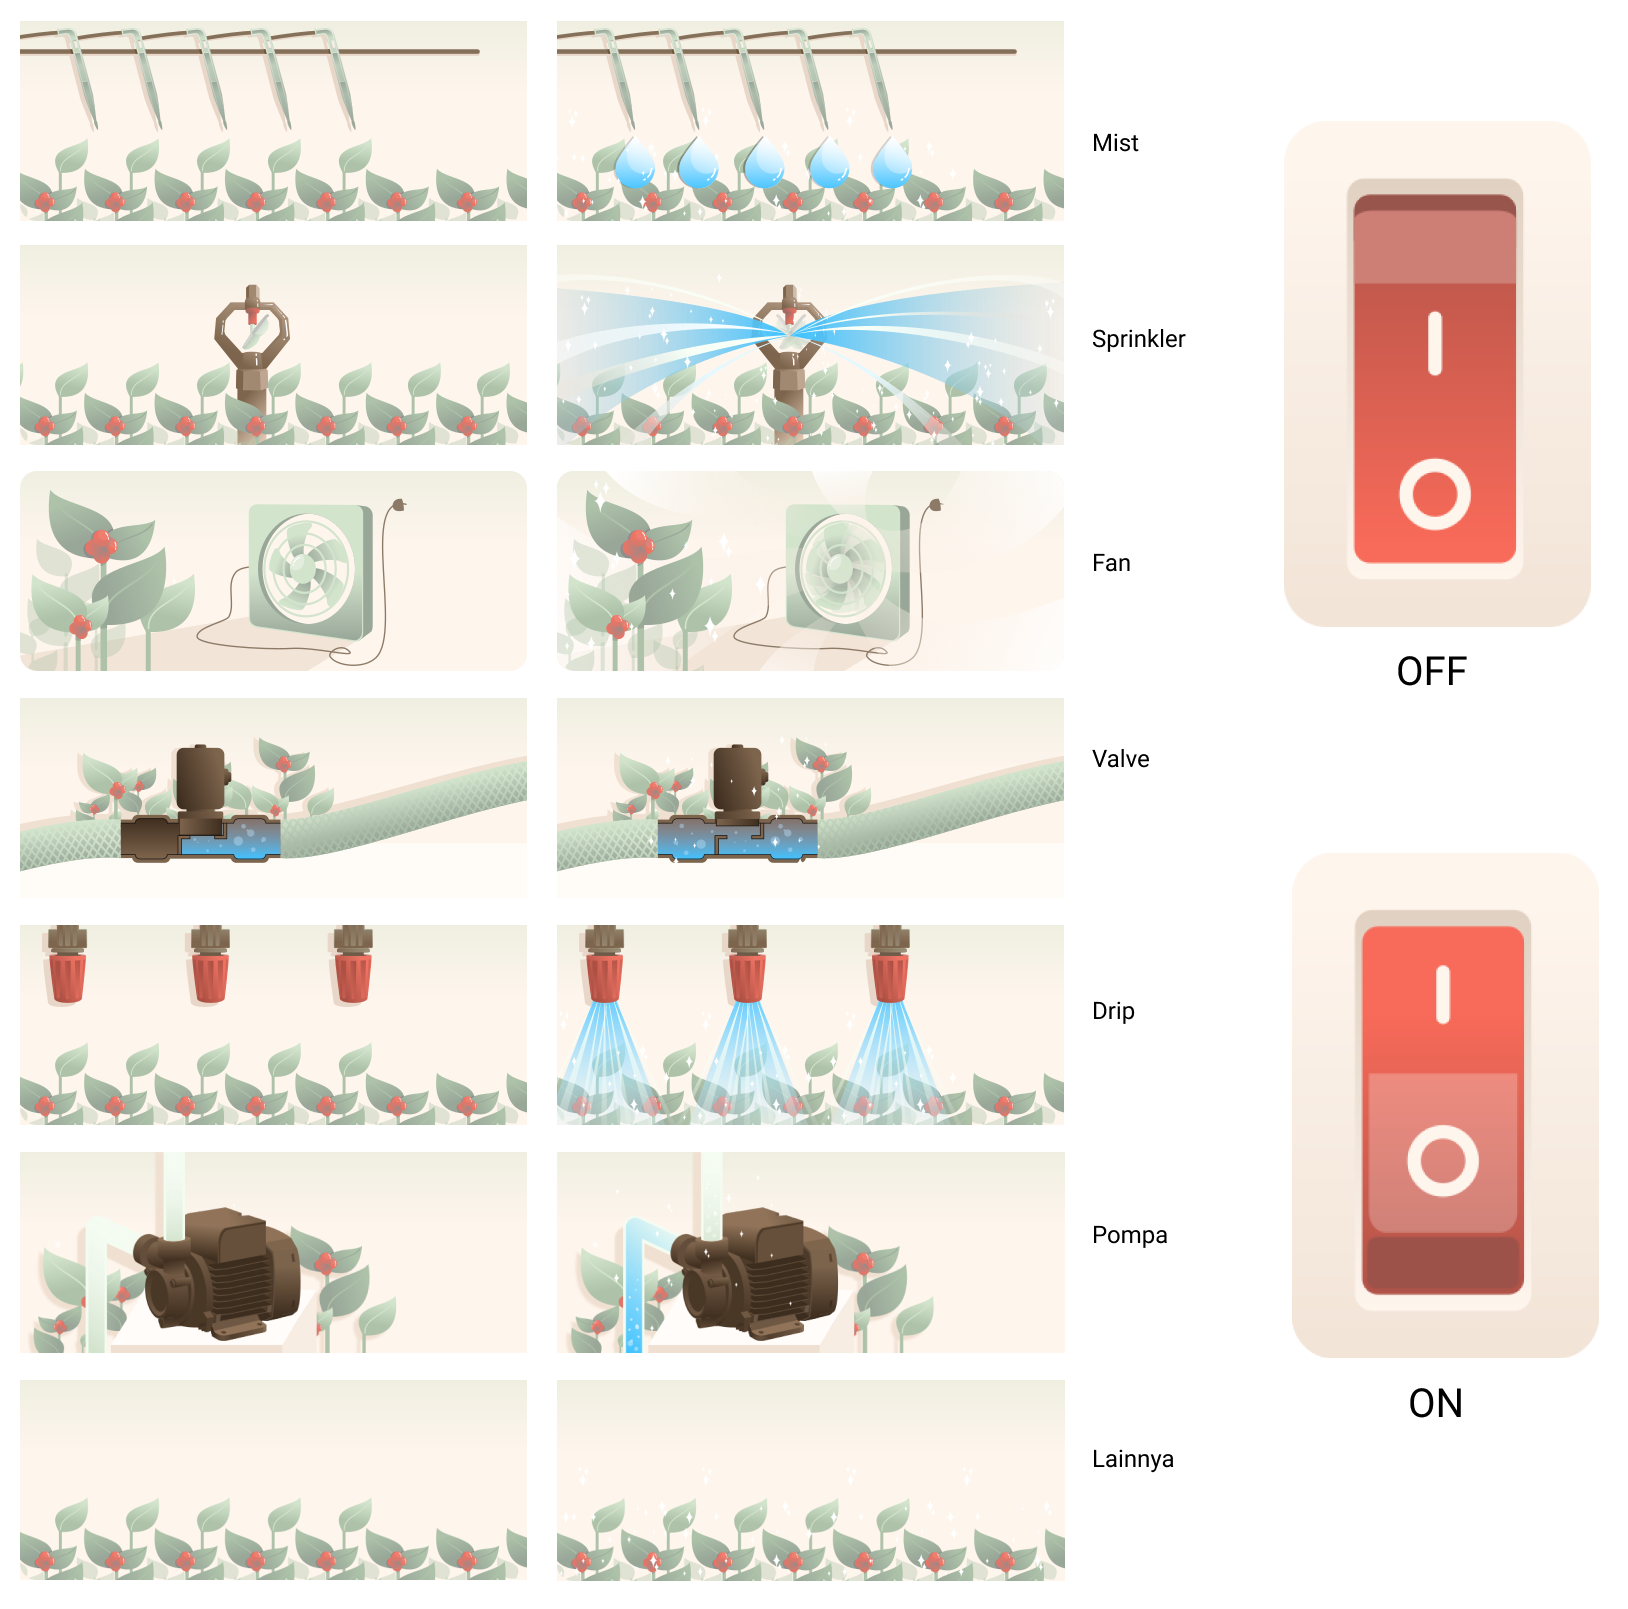
\includegraphics[width=7cm]{images/UI/Frame 1.png}
      %       \caption{\textit{Flow Chart} Alur Pengembangan Tugas Akhir}
      %   \end{figure}
         \item Metode pengembangan yang digunakan adalah \textit{Rapid Application Development} (RAD)
         \item Cara pengumpulan data yang digunakan adalah kuesioner dan pengujian\\
      \end{enumerate}

      \section{Ilustrasi Perhitungan Metode}
      Pengujian penerimaan aplikasi oleh pengguna dilakukan dengan menggunakan metode pengujian UAT, skala 
      \emph{likert} digunakan untuk menilai bobot dari hasil pengisian kuesioner. Bobot jawaban kuesioner \cite{kuantitatif}
      dapat dilihat bada Tabel 3.1
      \begin{table}[ht]
         \centering
         \caption{Bobot nilai jawaban}
         \begin{tabular}{|>{\raggedright}p{5cm}|p{2.5cm}|>{\raggedright}p{5cm}|}
          \hline
          \multicolumn{1}{|c}{\bfseries Jawaban} & \multicolumn{1}{|c|}{\bfseries Bobot} \\ 
           \hline
         \begin{center}
            Sangat Setuju
         \end{center} &
            \begin{center}
               5
            \end{center}
              \tabularnewline
              \hline
         \begin{center}
            Setuju
         \end{center} &
               \begin{center}
                 4
            \end{center}
             \tabularnewline
           \hline
         \begin{center}
            Netral
         \end{center} &
               \begin{center}
                 3
            \end{center}
             \tabularnewline
           \hline
         \begin{center}
            Tidak Setuju
         \end{center} &
               \begin{center}
                2
            \end{center}
             \tabularnewline
           \hline
         \begin{center}
            Sangat Tidak Setuju
         \end{center} &
               \begin{center}
                1
            \end{center}
             \tabularnewline
           \hline
          \end{tabular}
         \end{table}
         \newline setelah dilakukan pengisian kuesioner dan didapatkan data responden, data kemudian diolah dengan cara mengalikan data jawaban dengan bobot yang tertera pada tabel 3.1. Kemudian hasil tersebut dijumlahkan dan hasilnya dikalikan dengan bobot jawaban :
         \begin{itemize}
            \item Jumlah skor responden Sangat Setuju (SS)  = Total x 5 = nilai SS
            \item Jumlah skor responden Setuju (S)  = Total x 4 = nilai S
            \item Jumlah skor responden Netral (N)  = Total x 3 = nilai N
            \item Jumlah skor responden Tidak Setuju (TS)  = Total x 2 = nilai TS
            \item Jumlah skor responden Sangat Tidak Setuju (STS)  = Total x 1 = nilai STS
         \end{itemize}
         Maka akan diketahu jumlah skor total = nilai SS + nilai S + nilai N + nilai TS + nilai STS
         \\\newline Setelah didapatkan jumlah skor total, selanjutnya mencari nilai terendah dan tertinggi. Misalnya ada 5 orang responden, maka dapat dihitung:
         \begin{itemize}
            \item Nilai terendah = 5 x jumlah pertanyaan x 1 = (jika jawaban STS semua)
            \item Nilai tertinggi = 5 x jumlah pertanyaan x 5 = (jika jawaban SS semua)
         \end{itemize}
         \noindent Setelah diperoleh skor total, maka penilaian tingkat penerimaan oleh pengguna pada aplikasi dapat dihitung dengan menggunakan rumus berikut \cite{kuantitatif}:
         \begin{equation}
            P = \frac{f}{n} \times 100\%
         \end{equation}
         \noindent Keterangan :
         \\P = Persentase
         \\n = Jumlah responden
         \\f = Frekuensi jawaban\\

         \begin{table}[ht]
            \centering
            \caption{Nilai Presentase}
            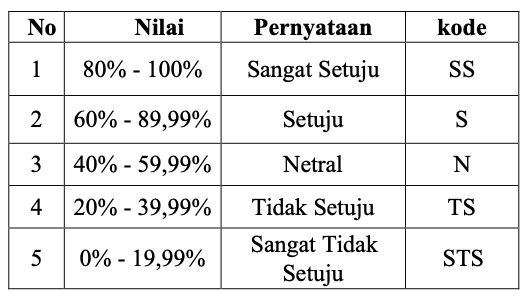
\includegraphics[width=8cm]{images/bab 3/table presentase.png}\\
            \end{table}
         \noindent Hasil pengujian UAT merepresentasikan pengujian penerimaan oleh pengguna, berdasarkan pengujian penerimaan tersebut ditarik kesimpulan apakah aplikasi yang telah diuji dapat diterima atau tidaknya oleh pengguna. Presentase yang sudah diolah diklasifikasikan berdasarkan skala penilaian berikut \cite{kuantitatif} : 
         \begin{figure}[ht]
            \centering
            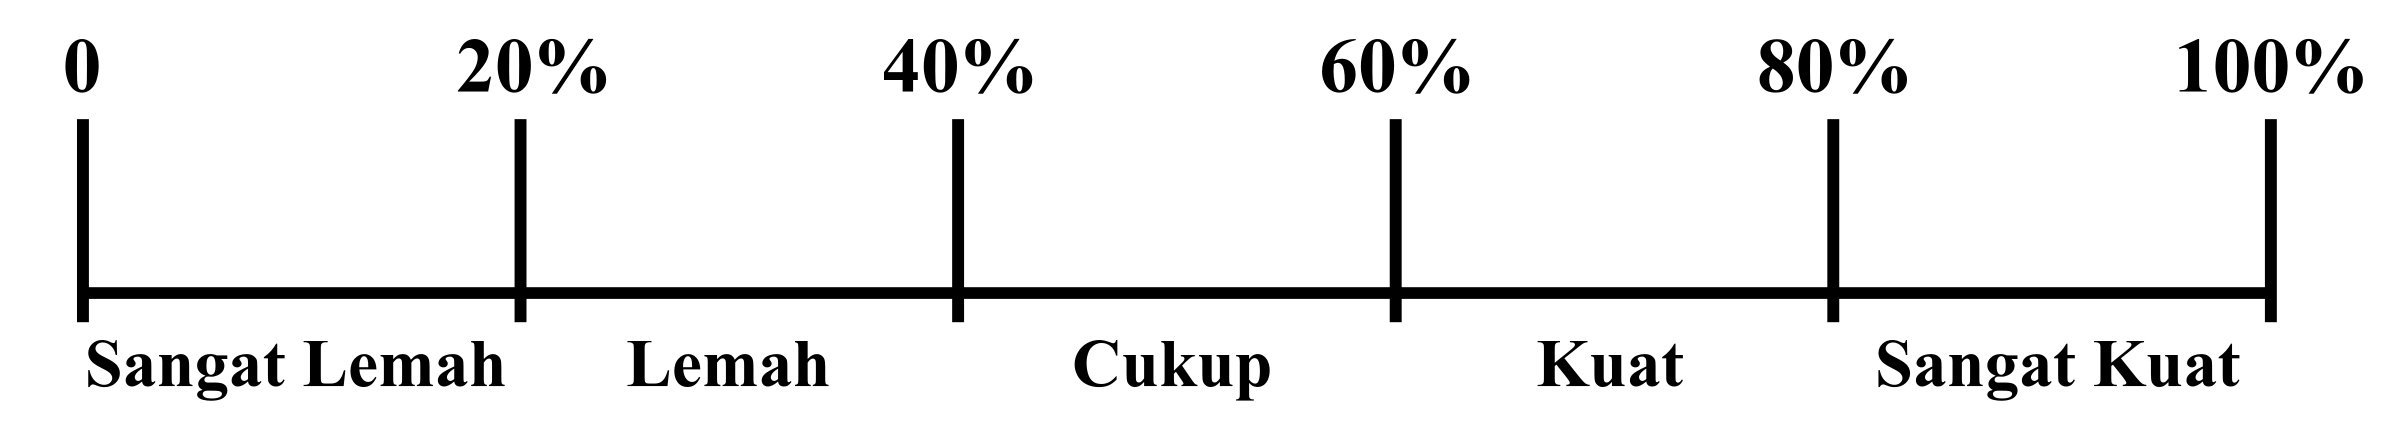
\includegraphics[width=11cm]{images/bab 3/skala.png}\\
            \caption{Skala Penilaian}
        \end{figure}
        \noindent \\Berikut nilai kesimpulan berdasarkan referensi \cite{kuantitatif} :
        \begin{table}[ht]
         \centering
         \caption{Nilai Kesimpulan}
         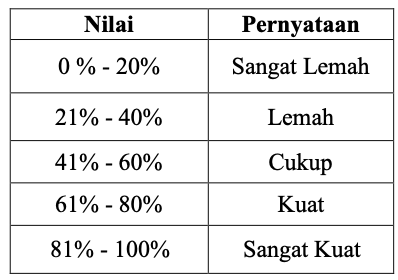
\includegraphics[width=8cm]{images/bab 3/Kesimpulan.png}\\
         \end{table}
         \noindent \\Jika nilai akhir dari perhitungan ternyata didapatkan hasil desimal, maka dapat dibulatkan ke nilai terdekat.\\
      
         \section{Rancangan Pengujian}
         Terdapat dua pengujian yang digunakan dalam penelitian ini. Pertama pengujian fungsionalitas dengan 
         menggunakan metode \emph{black box testing}, dan yang kedua menggunakan metode pengujian \emph{User 
         Acceptance Testing} (UAT) guna mengetahui tingkat penerimaan pengguna. Kedua pengujian tersebut akan
          dirancang komponen pengujiannya setelah penelitian sudah melewati proses pemodelan proses yakni tahap sebelum tahap pembuatan aplikasi dalam penelitian ini.\\
            % \subsection{\emph{Black box testing}}
            % Karena aplikasi dirancang hanya untuk satu jenis pengguna (pelanggan), maka pengujian fungsionalitas tertera hanya kepada 1 role pengguna. Pengujian nantinya dirancang setelah penelitian berjalan, sehingga diketahui komponen apa saja yang perlu diuji secara fungsionalitas.\\
            %    % \subsubsection{Pengujian Halaman Login}
            %    % \subsubsection{Pengujian Bagian Menu Alat}
            %    % \subsubsection{Pengujian Halaman Home}
            
            % \subsection{Pengujian \emph{User Acceptance Testing} (UAT)}

   
   \end{justify}
   
\end{flushleft}

% \vspace{5cm}
% \noindent \textbf{CONTOH Penulisan}
% \section{Analisa Sistem}

% \subsection{Analisa Sistem Saat Ini}
% Analisa sistem pendukung keputusan dalam penentuan penjurusan dibuat oleh peneliti dalam bentuk use case diagram yang mewakili secara sederhana dan bisa dijadikan sebagai bahan dalam evaluasi sistem yang berjalan, sehingga sistem dapat terlihat tanpa harus mengetahui secara detail prosedur yang berjalan.
% \begin{figure}[ht]
% 	\centering
% 	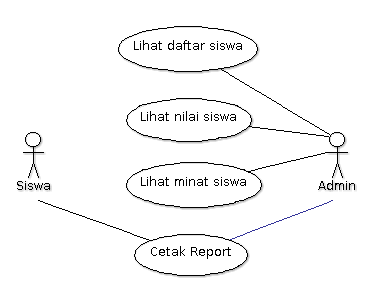
\includegraphics[width=10cm]{images/UseCaseDiagramSistemSaatIni}
% 	\caption{Use Case Diagram Analisa Sistem Saat Ini}
% \end{figure}

% \newpage
% \noindent Dibawah ini merupakan deskripsi dari use case yang sedang berjalan:
% \begin{enumerate}[nolistsep,leftmargin=0.5cm]
% \item \textit{Admin} melihat daftar siswa.
% \item \textit{Admin} melihat nilai setiap siswa.
% \item \textit{Admin} melihat minat setiap siswa.
% \item \textit{Admin} mencetak hasil keputusan.
% \item Siswa melihat laporan penjurusan yang telah dicetak oleh \textit{admin}
% \end{enumerate}

% \subsection{Evaluasi Sistem Saat Ini}

% \begin{table}[ht]
% \centering
% \caption{Permasalahan dan Solusinya}
% \begin{tabular}{|>{\raggedright}p{5cm}|p{2.5cm}|>{\raggedright}p{5cm}|}
%  \hline
%  \multicolumn{1}{|c}{\bfseries Masalah} & \multicolumn{1}{|c|}{\bfseries Aktor} & \multicolumn{1}{c|}{\bfseries Solusi} \\ 
%   \hline
% \begin{enumerate}
%    	\item Masalah masalah masalah Masalah masalah masalah Masalah masalah masalah Masalah masalah masalah.
%    	\item Masalah masalah masalah Masalah masalah masalah Masalah masalah masalah Masalah masalah masalah.
%    	\item Masalah masalah masalah Masalah masalah masalah Masalah masalah masalah Masalah masalah masalah.
%    \end{enumerate} &
%    \begin{enumerate}
%   	\item Aktor 1
%   	\item Aktor 2
%   \end{enumerate} &
%   \begin{enumerate}
%   \item Solusi solusi solusi Solusi solusi solusi Solusi solusi solusi Solusi solusi solusi Solusi solusi solusi.
%   \item Solusi solusi solusi Solusi solusi solusi Solusi solusi solusi Solusi solusi solusi Solusi solusi solusi.
%   \item Solusi solusi solusi Solusi solusi solusi Solusi solusi solusi Solusi solusi solusi Solusi solusi solusi.
%   \end{enumerate}
%      \tabularnewline
%   \hline
%  \end{tabular}
% \end{table}

% \subsection{Model yang Diusulkan}

% \subsection{Acitivity Diagram yang Diusulkan}

% \subsection{Perancangan Prosedur Sistem}

% \subsubsection{Use Case Diagram}

% \subsubsection{Activity Diagram}
% \begin{enumerate}[nolistsep,leftmargin=0.5cm]
% \item \textit{Activity diagram} satu

% \begin{enumerate}[label=\alph*.]
% 	\item Item 1.
% 	\item Item 2.
% 	\end{enumerate}
% \item Dua
% \end{enumerate}

% \subsubsection{Class Diagram}

% \subsubsection{Sequence Diagram}

% \subsection{Perancangan Antarmuka (Interface)}

\newpage